\documentclass[12pt, letterpaper]{article}
\usepackage{setspace} 
\usepackage{graphicx} 
\usepackage{dcolumn}
\usepackage{placeins}
\usepackage{natbib}
\usepackage{subcaption}
\usepackage{float}
\usepackage{lipsum} 
\usepackage{mathpazo}
\usepackage{hyperref}
\usepackage{amsmath}
\usepackage{pdflscape}
\bibliographystyle{econ}
\hypersetup{
    colorlinks=true,%    linkcolor=blue,    filecolor=magenta,      
    urlcolor=cyan,
    citecolor=blue
}

\usepackage[letterpaper, margin=1in]{geometry}


\begin{document}
\title{Measuring Knowledge Capital Risk: Evidence from firm 10-Ks}
\author{Pedro H. Braz Vallocci \footnote{Ph.D. candidate in Economics, University of California, Santa Cruz} 
\footnote{I am very grateful to my advisor, Galina Hale, for her continuous support throughout my Ph.D. I also thank Alonso Villacorta, Grace Gu, John Fernald, Michael Leung, Brenda Samaniego de la Parra, Chenyue Hu, Roberto Mauad, Bhavyaa Sharma, Ted Liu, Harrison Shieh, and the UCSC Macro Workshop participants for all their valuable comments.}} % 

\newcommand{\ffo}{dicfullmc10thr10defnob40noa1_4t}

\newcommand{\insertfigure}[3]{
\begin{figure}[H]
  \centering
  \includegraphics[width=#3\textwidth]{\ffo/#1}
  \caption{#2}
  \label{fig:#1}
\end{figure}
}

% TODO
% - Iterate with new priors until you find a fixed point. List key phrases: knowledge, innovation...
% - A better idea would be to choose number of topics with perplexity or something alike.
% - Elaborate on why existing measures are not good enough.
% - Move on to the rest of the paper to not get bogged down in the end. Take a break, come back.
% - Keep talking to Michael
% - Fin institutions are different in debt/assets and productivity measures. Not sure if I need to remove them or not. Maybe keep them and do a robustness test. 
% - Michael: use the ground truth somewhere. 

\newcommand{\tkk}{$Topic_{kk}$ }

\maketitle 

\begin{center}
For the latest version of this paper, click \href{https://github.com/pbrazval/jmdocs/blob/main/brazvallocci_jmp.pdf}{here}.
\end{center}

\begin{abstract}
    This study proposes a novel measure of yearly firm-level R\&D-related risks, by performing an LDA analysis of self-reported risk factors disclosed in firms' 10-Ks.  Higher levels of R\&D risks are associated with distinctive and higher levels of volatility and kurtosis in stock returns, consistent with previous literature on the R\&D anomaly and the expectation of increased tail risk for R\&D ventures. \newline \textbf{\indent Keywords:} Innovation, firm risk factors, productivity, intangible capital, natural language processing, asset pricing \newline \textbf{\indent JEL classification:} C43, C55, D2, E22, G11, O3
\end{abstract}

\newpage 

\onehalfspacing 

\section{Introduction}



% Galina's feedback: should include:


% 1) What is the problem
% 2. What is the current answer
% 3. What do you add in this paper.

% Knowledge-capital heavy are known to have different 

% Open: Moved from the bottom following Galina's feedback (that this part needs to be in the first page). Can be better mixed with the text above/below

The transition towards a service- and knowledge-based economy has been accompanied by a sharp increase in intangible assets. Knowledge capital, conceptualized as the aggregate of a firm's investments in research and development (R\&D), has become an increasingly significant factor in the valuation of firms \citep{Belo2019-iz}. Firms endeavor to foster innovation through research, aiming to generate intellectual property that may lead to breakthroughs and augment cash flows. Concurrently, firms face the challenges of competition and product obsolescence, which can symmetrically induce sudden devaluations. The episodic nature of innovation implies that firms with substantial knowledge capital are likely to experience more volatile valuations. 

However, the existing literature has predominantly attempted to correlate the risk associated with knowledge capital to a firm's R\&D or patent intensity \citep{Andrei2019-bh}. Such classifications overlook the reality that the efficacy with which firms convert R\&D into tangible innovations—and consequently into increased cash flows—is both industry-specific and firm-specific. Moreover, patenting activities are recognized to be unevenly distributed across industries and firm sizes \citep{mezzanotti2023innovation, Li2020-xc}. 

Within this framework, several pertinent questions arise: Can we more accurately discern knowledge-related risks by conducting textual analysis of the risk factors delineated in firms' annual reports? Furthermore, if it is possible to identify knowledge-intensive firms in this manner, does this insight impact the way market participants value these entities? In essence, is there a differential in the market's risk assessment for firms with heavy knowledge capital compared to their less knowledge-intensive counterparts? This paper proposes a methodology to identify firms that are vulnerable to knowledge capital-related risks, relying on a topic analysis (LDA) of the risk factors disclosed in their annual reports. Further, the paper quantifies these risks through an examination of firms' concurrent return patterns.

Spending on intangible assets is an investment since it reduces current consumption to increase future consumption \citep{Corrado2009-kd, Corrado2009-hk}. Among the components of a firm's intangible capital are knowledge capital, brand capital, and organization capital.  In this context, \emph{brand capital} is defined as a firm's accumulated expenses in advertising \citep{Belo2019-iz}; \emph{organization capital}, as the set of an enterprise's unique systems and processes %, being positively correlated with the firm's managerial quality scores 
\citep{Eisfeldt2013-ad, Bloom2007-gl}; and \emph{knowledge capital}, as a firm's accumulated investments in R\&D.
%most notably in research and development

Accumulated R\&D expenses are considered an integral part of firm's capital in supply-side models such as \cite{Belo2013-ys}, accounting for an increasing share of public firms' valuation. Along these lines, \cite{Hall2001-ni, McGrattan2001-kc, Vitorino2014-yd, Eisfeldt2020-ec, Li2014-zp} confirm that intangible capital matters for aggregate stock market valuations and, more specifically, firm-level valuations. \cite{Corrado2009-kd} estimated total intangible capital in 2003 to be 3.6 trillion, half of which as scientific and non-scientific R\&D capital. \cite{Crouzet2022-ic} found that the omission of knowledge capital and its associated rents can explain up to 2/3 of the investment gap (the difference between marginal $q$ and average $Q$) in R\&D intense sectors such as Healthcare and Chemicals. On another note, R\&D expenditures are considered as intermediate expenses that can spur growth in models with expanding varieties \citep{Romer1990-tw} and quality ladders \citep{Grossman1991-pz, Atkeson2019-wz}.
%Notably, this form of capital exhibits a distinct risk profile compared to tangible, physical capital. For instance, companies heavily reliant on knowledge capital are more susceptible to the loss of critical personnel and modifications in patent enforcement. 



%  Moreover, endogenous growth models, such as models with expanding varieties \citep{Romer1990-tw}, and with quality ladders \citep{Grossman1991-pz, Atkeson2019-wz}, imply that research expenses can spur growth. Even though the two latter models consider R\&D as intermediate expenses, supply-side valuation models such as \cite{Belo2013-ys} argue that not only quasi-fixed physical capital and labor inputs but also knowledge and brand capital can determine a firm's market value. 



%However, equating the omission of intangible and knowledge capital to a mere mismeasurement of a firm's book value is misleading since intangible capital has unique characteristics and thus cannot be lumped together with physical capital. \cite{Autor2020-rw, Unger2019-ip} shed light on a "scale-biased technological change" in R\&D-heavy firms. Greater output scalability, the absence of geographical constraints for input sourcing or output distribution, and the greater importance of network effects lead to a "winner-takes-most" outcome in some industries (i.e., an uneven market power distribution) and a declining labor share, consistent with \cite{Barkai2020-gi}.
%
%Moreover, R\&D-driven technological innovation, while generating research externalities in the form of knowledge available to the rest of society, may also be a force for creative destruction \citep{Schumpeter1939-er} if it leads to mere resource reallocation across firms. Therefore, it is not evident that private-led innovation increases aggregate output. \citep{Kogan2017-fx, Garcia-Macia2019-mg} show that innovation has a net effect of accelerating aggregate output and that own-product improvements by incumbents are more important than creative destruction.
%
%R\&D-intensive firms are also more likely to offshore profit shifting, i.e., to license their intellectual property rights to offshore subsidiaries in order to accrue derived profits at tax-havens. Compared to non-R\&D-intensive firms (e.g., construction), it is easier to decouple the physical location of intellectual property production from its point of sale. Offshore profit shifting has grown since the 2000s, which coincides with the beginning of the productivity growth slowdown \citep{Fernald2015-io}. Adjusting for offshore profit shifting adds 2.1 log percentage points to R\&D-heavy firms, which is ten times larger than for non-R\&D. Labor productivity in R\&D-intensive firms has also grown much faster than in non-R\&D firms \citep{Guvenen2021-yh}.

The riskiness of intangible assets differs systematically from tangible ones \citep{Hansen2005-xe}. \cite{Eisfeldt2013-ad} point out that shareholders cannot entirely appropriate the cash flows from the key talent of the firm since the firm must always compensate key talent by its outside option. \cite{Eisfeldt2018-iy} shows that key talent partially owns the cash flow from intangible capital in the form of equity, finding that almost 40\% of compensation to high-skilled labor happens as equity-based pay. Finally, \cite{Ai2019-wd} predicts that collateralizable assets, which do not include some categories of intangibles, provide insurance against aggregate shocks in the economy and should earn a lower expected return.

Knowledge capital's risk characteristics set it apart from other forms of intangible capital. Firms invest on research to increase their future earnings, but not all innovations come to fruition. For example, research conducted by a pharmaceutical firm can lead to successful new drugs that lead to patent rents for several years or to no result at all. The presence of innovation-driven jumps in cash flow is related to an increased empirical dispersion of Tobin's q, and also helps explain why the relatxion between Tobin's q and aggregate investment has become tighter since the mid-1990s \citep{Andrei2019-bh}. 

An example of volatility caused by R\&D investments in a firm is shown in Figure \ref{fig:amazon_nov01}.

\insertfigure{amazon_nov01}{Text}{0.9}

Besides the uncertainty of research investments, a firm is also susceptible to writing off part of its knowledge capital due to obsolescence, e.g., when it narrowly loses a patent race \citep{Peters2017-fl}. Such competitive forces lead to R\&D capital depreciation. Depreciation rates vary over time and according to individual industry technological and competitive environments \citep{Li2020-xc}. Besides varying between industries, it is expected that depreciation rates vary across firms in the same industry, since firms' ability to materialize research into innovation and additional cash flow is also expected to be random, varying with managerial processes, employees' skills, and regulation-related uncertainty.

Knowledge capital heavy firms also are especially vulnerable to loss of key talent. \cite{Eisfeldt2013-ad} find that firms are more likely to list ``loss of key talent" as a risk factor in their 10-K reports when they have high organization capital. Firms vulnerable to loss of key talent are especially susceptible to immigration-related risks, e.g., the H-1B visa annual quota shortages \citep{Peri2015-qt}. 
%It makes sense that the same pattern is valid for knowledge capital heavy firms, which are highly dependent on specialized and scarce workforce. 

A prominent reliance on R\&D may also entail a different financial risk profile. \cite{Li2011-ay} find that the riskiness of a financially constrained firm increases with its R\&D intensity. Additionally, young, R\&D-intensive firms frequently face challenges in securing debt finance due to the unpredictable and fluctuating returns on R\&D, and the potential adverse selection and moral hazard in the R\&D financing market. Notably, fluctuations in the supply of equity finance were instrumental in shaping the R\&D surge of the 1990s \citep{Brown2009-zp}, pointing to a shared risk factor among these firms.

%. The H-1B visa, introduced with the Immigration and Nationality Act of 1990, established temporary renewable visas for college-educated specialty professional workers, most of whom work in STEM occupations. \cite{Peri2015-qt} shows that the growth in foreign-STEM workers may explain between 10 and 25\% of the aggregate productivity growth and 10\% of skill-bias growth between 1990 and 2010.

%Following previous literature on time-varying disaster risks, such as \cite{Gabaix2012-kw, Barro2006-pt, Rietz1988-ds, Gourio2012-nt} shows that increases in the risk of an economic disaster can lead to an increase in risk premia and a decrease in unemployment and output. My work will develop upon \cite{Gourio2012-nt} to consider a knowledge capital heavy economy, and investigate if agents are pricing in the risk of sudden drops in the efficiency of knowledge investment (e.g., due to shortage of skilled workforce) or sudden firm-specific write-offs ("disasters") of knowledge capital (e.g., due to weakening in patent laws).

%%%%%%%%%%%%%%%%%%%%%%%%%%%%%
% Why not sufficient
% R\&D
The current methods of identifying knowledge capital related risk across firms, deriving from uncertain outcomes of research, use proxies (accumulated R\&D, SG\&A, patent wealth) that fail to accurately describe potential volatilities in cash flows. A possible approach might involve tying knowledge capital risk to a firm's knowledge capital, normalized by its assets or another variable. However, a significant limitation is the inconsistent R\&D reporting standards across industries and firms. This inconsistency is exacerbated by some firms not disclosing their R\&D expenditure in annual reports.  Similarly, methods that merely accumulate R\&D expenses  to characterize the knowledge intensity of a firm, using the perpetual inventory method, ignore that depreciation is random and unique to each firm.

%SG&A
Another possible, and similar, approach involves tying knowledge capital risk to a firm's total intangible assets instead, typically through indirect measures like Selling, General and Administrative expenses (SG\&A). However this measure is by nature prone to considerable measurement error and includes not knowledge-related components, such as organizational capital and brand capital. This can blur the distinction between knowledge-heavy and non-knowledge-heavy firms.

%Patents
Lastly, relying on patents as a measure of a firm's knowledge intensity only tells part of the story. While patents reflect the final outcomes of R\&D investments, they do not account for the internal learning processes that take place within firms, thus potentially undervaluing those that invest heavily in internal knowledge development, even if they do not have a high patent output. Additionally, measures of patent activity, such as the one in \cite{Kogan2017-fx}, are not flawless indicators of the risks associated with R\&D-centric firms. Large firms and firms in specific industries are more prone to protecting their intellectual property, which shows that patent distribution does not directly mirror the exposure to knowledge capital risks \citep{mezzanotti2023innovation}.

\citet{Kogan2017-fx} demonstrate that the companies' market value surges within the following three days of the filing of potentially lucrative patents, that is, patents that have the potential to amplify a firm's revenue streams while simultaneously stifling competition. Yet, one must ponder whether the stock market, outside patent-filing moments, also internalizes the inherent risks of devoting a significant part of investments to a risky innovation process.

\section{Data}

\subsection{10-K data}

I retrieve a total of  121,839 annual reports (10-Ks) for all U.S. publicly listed firms since 2013 from the EDGAR (Electronic Data Gathering, Analysis, and Retrieval) system, the Securities and Exchange Commission's electronic database used for the submission and public disclosure of financial statements and other reports filed by American publicly listed companies. A 10-K is a comprehensive document that provides an overview of the company's financial performance and operations over a year, offering a detailed picture of a company's business.  To ensure transparency and accuracy, laws and regulations strictly prohibit companies from making false or misleading statements in their 10-Ks. Additionally, under the Sarbanes-Oxley Act, enacted to enhance corporate transparency and accountability, a company's Chief Financial Officer (CFO) and Chief Executive Officer (CEO) are required to certify the accuracy of the 10-K (\cite{SEC_Office_of_Investor_Education_and_Advocacy2011-tw}).

Within the 10-K form, item 1A (``Risk Factors") mandates registrants, when applicable, to disclose in plain English risk factors that make investments in the firm speculative or risky. The discussion must be logically organized, risks must be adequately described, and the reasons why risks affect the registrant must be explained. Specifically, presenting risks that could apply generically to any registrant is discouraged (17 CFR § 229.105).  Norms enforcing text structure, writing style, and readability also apply, ensuring that the risk factors are communicated effectively to all stakeholders, including those without specialized financial or legal knowledge (17 CFR § 230.421).

Reporting risk factors is mandatory for most firms; however, there are exceptions for asset-backed issuers and smaller reporting companies. Asset-backed issuers are defined as issuers whose reporting obligation arises from either the registration of an offering of asset-backed securities under the Securities Act or the registration of a class of asset-backed securities. 

\subsubsection{Filtering 10-K reports}
\label{sec:filt10k}
Following \cite{Golubov2019-ku, Stambaugh2016-eb}, I filter firms by considering only ordinary common shares (CRSP share codes 10 and 11), traded on NYSE, AMEX, and NASDAQ exchanges (CRSP exchange codes 1, 2, and 3). Additionally, I exclude firms whose prices are less than \$5 in 2016 dollars, to avoid micro-structure effects. 

Furthermore, non-reporting firms must also be filtered out. Firms that are not required to disclose risk factors either leave Item 1A empty or write a distinctively short placeholder text specifying that, due to their nature, they are not required to disclose risk factors. Consequently, there is an abnormal frequency of 10-K filings with a significantly low number of words, as depicted in Figure \ref{fig:cdf}. In subsequent stages, 1A texts with an insufficient word count are discarded. The threshold adopted was 200 words. 

The total count of filtered firms by year is shown in Table \ref{tab:file_counts}. A total of 40,174 firm-year combinations are represented in the final topic map.

The next step is to convert each text in the corpus to a bag-of-words format, detailed in Appendix A.

\begin{table}[!htbp] \centering 
  \caption{File Counts by Year} 
  \label{tab:file_counts} 
\begin{tabular}{@{\extracolsep{5pt}} D{.}{.}{-3} D{.}{.}{-3} D{.}{.}{-3} } 
\\[-1.8ex]\hline 
\hline \\[-1.8ex] 
\multicolumn{1}{c}{Year} & \multicolumn{1}{c}{Total\_1As} & \multicolumn{1}{c}{Filtered} \\ 
\hline \\[-1.8ex] 
\multicolumn{1}{c}{2006} & \multicolumn{1}{c}{5685} & \multicolumn{1}{c}{2466} \\ 
\multicolumn{1}{c}{2007} & \multicolumn{1}{c}{6445} & \multicolumn{1}{c}{2714} \\ 
\multicolumn{1}{c}{2008} & \multicolumn{1}{c}{6931} & \multicolumn{1}{c}{2305} \\ 
\multicolumn{1}{c}{2009} & \multicolumn{1}{c}{8244} & \multicolumn{1}{c}{2190} \\ 
\multicolumn{1}{c}{2010} & \multicolumn{1}{c}{8122} & \multicolumn{1}{c}{2290} \\ 
\multicolumn{1}{c}{2011} & \multicolumn{1}{c}{8019} & \multicolumn{1}{c}{2356} \\ 
\multicolumn{1}{c}{2012} & \multicolumn{1}{c}{7797} & \multicolumn{1}{c}{2316} \\ 
\multicolumn{1}{c}{2013} & \multicolumn{1}{c}{7560} & \multicolumn{1}{c}{2401} \\ 
\multicolumn{1}{c}{2014} & \multicolumn{1}{c}{7560} & \multicolumn{1}{c}{2518} \\ 
\multicolumn{1}{c}{2015} & \multicolumn{1}{c}{7531} & \multicolumn{1}{c}{2528} \\ 
\multicolumn{1}{c}{2016} & \multicolumn{1}{c}{7196} & \multicolumn{1}{c}{2431} \\ 
\multicolumn{1}{c}{2017} & \multicolumn{1}{c}{6896} & \multicolumn{1}{c}{2394} \\ 
\multicolumn{1}{c}{2018} & \multicolumn{1}{c}{6804} & \multicolumn{1}{c}{2418} \\ 
\multicolumn{1}{c}{2019} & \multicolumn{1}{c}{6683} & \multicolumn{1}{c}{2404} \\ 
\multicolumn{1}{c}{2020} & \multicolumn{1}{c}{6531} & \multicolumn{1}{c}{2332} \\ 
\multicolumn{1}{c}{2021} & \multicolumn{1}{c}{6936} & \multicolumn{1}{c}{2308} \\ 
\multicolumn{1}{c}{2022} & \multicolumn{1}{c}{6899} & \multicolumn{1}{c}{1885} \\ 
\hline \\[-1.8ex] 
\end{tabular} 
\end{table} 

\subsection{Firm-level data}

Firm-level data is retrieved from CRSP-Compustat's Fundamentals Annual database.

\subsection{Intangible and knowledge capital data}

The data on intangible and knowledge capital is sourced from WRDS, based on the measurement methodology outlined by \cite{Peters2017-fl}, which employs the perpetual inventory method on firms' expenses on SG\&A (selling, general, and administrative expenses). Intangible capital is defined as the estimated replacement cost of a firm's intangible assets. Knowledge capital, a subset of intangible capital, specifically represents the replacement cost of the firm's knowledge assets derived from research and development activities, as reported under R\&D in their balance sheets.

\subsection{Stock returns data}

Stock return data is sourced from the Center for Research in Security Prices (CRSP). As outlined in Section \ref{sec:filt10k}, stocks priced below \$5, as measured by their June average in each year, are excluded from the analysis. To adjust for price changes over time, the Consumer Price Index for All Urban Consumers (CPI-U), obtained from the Federal Reserve Economic Data (FRED) database, is employed for inflation adjustment. Stock return data is retrieved in multiple frequencies (daily, weekly, monthly). 

Fama-French factors such as SMB and HML; risk-free rates (one-month Treasury bill rate, obtained from Ibbotson Associates); and excess market returns are retrieved from Kenneth French's website.


\subsection{Patent data}

The economic value of each patent filed by individual firms is obtained from the dataset available on Dimitris Papanikolaou's website, according to the methodology described in \cite{Kogan2017-fx}. This value represents the private economic value of each patent, calculated based on the firm's current market capitalization and the idiosyncratic return of the firm's stock around the time of the patent's issuance. This calculation takes into account the need to exclude market-wide movements and potential measurement errors to isolate the specific impact of the patent issuance on the firm's value.

Patent values are accumulated on an annual basis to construct a metric representing the total added patent value for each firm in each respective year. Missing data for added patent value are substituted by 0. Patent values are deflated to 1982 (million) dollars using the CPI.

\subsection{Other data}

Industry-specific labor skill data is sourced from Frederico Belo's website, following the definition provided by \cite{Belo2017-qi}. In their study, the skill level within an industry is quantified as the proportion of employees engaged in occupations necessitating extensive training and preparation, defined as occupations with a Specific Vocational Preparation (SVP) level of 7 or higher. Industries are categorized using 4-digit NAICS codes. For the years post-2013, the established labor skill level as of 2013 is applied.

Databases indexed with different keys (such as CRSP, PERMNO, or GVKEY) were merged using the CRSP-Compustat Merged Database link table.


\begin{landscape}
\begin{table}[!htbp] \centering 
  \caption{Descriptive Statistics} 
  \label{tab:descstat} 
\begin{tabular}{@{\extracolsep{5pt}} m{9cm}cccccc} 
\\[-1.8ex]\hline 
\hline \\[-1.8ex] 
 & Mean & Median & St. dev. & Min & Max & n \\ 
\hline \\[-1.8ex] 
topic\_kk & $0.10$ & $0$ & $0.25$ & $0$ & $1$ & $40,173$ \\ 
topic\_finl & $0.24$ & $0.05$ & $0.36$ & $0$ & $1$ & $40,173$ \\ 
topic\_sw & $0.29$ & $0.14$ & $0.34$ & $0$ & $1$ & $40,173$ \\ 
topic\_rawm & $0.36$ & $0.20$ & $0.37$ & $0$ & $1$ & $40,173$ \\ 
Skill & $0.33$ & $0.29$ & $0.18$ & $0.01$ & $0.76$ & $38,922$ \\ 
Annual patent value added & $226$ & $0$ & $2,048$ & $0$ & $87,430$ & $40,173$ \\ 
Total patent value accumulated (millions) & $6,905$ & $0$ & $49,944$ & $0$ & $1,162,766$ & $40,173$ \\ 
Total patent value / total assets & $0.38$ & $0$ & $1.70$ & $0$ & $116$ & $40,173$ \\ 
Annual patent value / total assets & $0.02$ & $0$ & $0.13$ & $0$ & $8.45$ & $40,173$ \\ 
Intangible capital (millions) & $2,656$ & $329$ & $11,253$ & $0$ & $278,772$ & $27,462$ \\ 
Knowledge capital (millions) & $427$ & $0$ & $3,012$ & $0$ & $78,910$ & $27,462$ \\ 
Total assets (millions) & $12,193$ & $1,342$ & $79,957$ & $0.42$ & $3,386,070$ & $34,485$ \\ 
\hline \\[-1.8ex] 
\end{tabular} 
\end{table} 

\end{landscape}

\section{Measuring knowledge capital risk at the firm level}

This paper introduces a novel measure for evaluating firm-level risks associated with R\&D ventures. R\&D is a crucial driver of innovation and firm value, with inherently uncertain outcomes. R\&D investment has option-like characteristics, whereby firms assess whether to continue or suspend R\&D based on anticipated cash flows (Berk, 2004; Leung, 2020). We highlight both the downside risks, such as regulatory rejections, lost patent races, or obsolescence of intellectual capital, and the upside potentials, exemplified by breakthrough patents that significantly boost firm earnings. 

In this paper, knowledge capital risk is defined as the unique form of risk that innovation-centric firms bear, particularly when their cash flow trajectories are influenced by the stochastic nature of research-induced innovations. This risk is inherent in the unpredictable timing and impact of such innovations on a firm's financial performance.

Methodologies for pattern detection in textual analysis encompass a range of techniques from simple pattern matching to more complex algorithmic constructions of term sets, as well as the identification of prevailing topics within textual data.

In light of these complexities, my approach will leverage Latent Dirichlet Allocation (LDA) to analyze the risk factor sections within firms' 10-K filings. This method will facilitate the extraction of dominant topics that are most indicative of knowledge capital risk. 

\subsection{Latent Dirichlet Allocation}

In this study, I use LDA, a topic modeling technique, to identify latent topics within firms' self-reported risk factors in a comprehensive corpus of 121,839 firm annual reports (10-Ks), covering a timespan from 2006 to 2022.


LDA is a generative statistical model that is widely employed for topic modelling within the field of natural language processing (NLP). LDA relies on the assumption that each document in a given corpus can be seen as a mixture of a certain number of latent topics, denoted as $k \in {1, ..., K}$, each of which carries a particular weight, $\omega_{i1}, ..., \omega_{iK}$. Each of these topics is assigned a word probability vector, $\mathbf{\theta}_k$, defining the likelihood of each word appearing under this topic \citep{Blei2003-ay}.

Under this model, if we denote $X_i$ as the vector of word counts with length $n_i$ in the $i$th document, the word distribution in a document is modeled as a multinomial distribution. The probability of $X_i$ can be written as:

\begin{equation}
X_i \sim Multinomial\left(n_i, \omega_{i 1} \theta_1+\cdots+\omega_{i K} \theta_K\right)
\end{equation}

%This equation represents the fact that the observed words in the document are generated by a mixture of topics, with each topic contributing to the document with a certain weight.

The output of an LDA operation is twofold: firstly, it generates a list of topics, with each topic represented as a collection of words. Secondly, it offers a weight distribution across these topics for each document, indicating the degree to which each topic is present in a given document.

It is important to note that LDA is an unsupervised learning method. This means that it operates without any predefined labels, instead learning and inferring patterns directly from the data. However, this also poses a challenge, since the topics generated might not necessarily align with any intuitive description, requiring therefore post-analysis interpretation. %This characteristic makes LDA a versatile tool, able to extract valuable insights from large and complex corpora of text data.

\subsection{Topic modeling}

Upon having the corpus and the dictionary, I employ LDA to endogenously generate topic loadings for the entire set of documents. During the model's configuration, I designate a parameter to specify the number of topics, represented as \(k\), and supply the model with the dictionary I previously created. Selecting an appropriate value for \(k\) is typically done \textit{ad hoc}, with the primary consideration being interpretability, as highlighted by Gentzkow (2019).

A representative output from this modeling approach can be viewed in Figure \ref{fig:wordclouds}.


\insertfigure{wordclouds}{A graphic representation of a four-topic model on firms' risk factors since 2006.}{0.7}

After merging a four-topic map between firms and topic intensities to firms' identifying data, I obtain a topic map as shown in Table \ref{tab:topic_map}.

\tiny

\begin{table}[!htbp] \centering 
  \caption{Sample of a topic map} 
  \label{} 
\begin{tabular}{@{\extracolsep{5pt}} D{.}{.}{-3} D{.}{.}{-3} D{.}{.}{-3} D{.}{.}{-3} D{.}{.}{-3} D{.}{.}{-3} } 
\\[-1.8ex]\hline 
\hline \\[-1.8ex] 
\multicolumn{1}{c}{Company\_Name} & \multicolumn{1}{c}{year} & \multicolumn{1}{c}{topic\_0} & \multicolumn{1}{c}{topic\_1} & \multicolumn{1}{c}{topic\_2} & \multicolumn{1}{c}{topic\_3} \\ 
\hline \\[-1.8ex] 
\multicolumn{1}{c}{AEROVIRONMENT INC} & \multicolumn{1}{c}{2010} & \multicolumn{1}{c}{0.822} & \multicolumn{1}{c}{0} & \multicolumn{1}{c}{0.141} & \multicolumn{1}{c}{0.036} \\ 
\multicolumn{1}{c}{AES CORP (THE)} & \multicolumn{1}{c}{2020} & \multicolumn{1}{c}{0.056} & \multicolumn{1}{c}{0.05} & \multicolumn{1}{c}{0.894} & \multicolumn{1}{c}{0} \\ 
\multicolumn{1}{c}{ARROWHEAD PHARMACEUTICALS} & \multicolumn{1}{c}{2016} & \multicolumn{1}{c}{0} & \multicolumn{1}{c}{0} & \multicolumn{1}{c}{0} & \multicolumn{1}{c}{0.997} \\ 
\multicolumn{1}{c}{BROOKDALE SENIOR LIVING INC} & \multicolumn{1}{c}{2015} & \multicolumn{1}{c}{0} & \multicolumn{1}{c}{0.475} & \multicolumn{1}{c}{0.406} & \multicolumn{1}{c}{0.114} \\ 
\multicolumn{1}{c}{ENTERPRISE FINL SERVICES CP} & \multicolumn{1}{c}{2008} & \multicolumn{1}{c}{0} & \multicolumn{1}{c}{0.999} & \multicolumn{1}{c}{0} & \multicolumn{1}{c}{0} \\ 
\multicolumn{1}{c}{II-VI INC} & \multicolumn{1}{c}{2017} & \multicolumn{1}{c}{0.791} & \multicolumn{1}{c}{0.012} & \multicolumn{1}{c}{0.197} & \multicolumn{1}{c}{0} \\ 
\multicolumn{1}{c}{KAISER ALUMINUM CORP} & \multicolumn{1}{c}{2014} & \multicolumn{1}{c}{0.34} & \multicolumn{1}{c}{0.037} & \multicolumn{1}{c}{0.623} & \multicolumn{1}{c}{0} \\ 
\multicolumn{1}{c}{NATURES SUNSHINE PRODS INC} & \multicolumn{1}{c}{2013} & \multicolumn{1}{c}{0.959} & \multicolumn{1}{c}{0} & \multicolumn{1}{c}{0} & \multicolumn{1}{c}{0.04} \\ 
\multicolumn{1}{c}{SOUTHWEST GEORGIA FINL CORP} & \multicolumn{1}{c}{2012} & \multicolumn{1}{c}{0} & \multicolumn{1}{c}{0.999} & \multicolumn{1}{c}{0} & \multicolumn{1}{c}{0} \\ 
\multicolumn{1}{c}{TECO ENERGY INC} & \multicolumn{1}{c}{2006} & \multicolumn{1}{c}{0} & \multicolumn{1}{c}{0} & \multicolumn{1}{c}{0.992} & \multicolumn{1}{c}{0} \\ 
\hline \\[-1.8ex] 
\end{tabular} 
\end{table} 

\normalsize

\section{Comparison to existing measures}

The concept of knowledge capital risk lacks an empirical "ground truth," a benchmark against which the accuracy of predictions or classifications can be validated, such as the VIX in \cite{Manela2017-lj}, used as ground truth to create a measure of news volatility dating back to 1890. Moreover, the construction of a comprehensive dictionary is complex, as the terminology can vary significantly across industries. For instance, the lexicon indicative of intellectual property concerns in pharmaceutical companies may frequently reference terms such as "clinical trials" or "regulatory compliance" within their annual reports.

In this section, I validate our text-based metric, $Topic_{kk}$, by cross-referencing it with established measures from prior literature. This assessment strengthens the reliability and relevance of our metric within the broader context of knowledge capital analysis.

Finally, I examine the implications of our findings for asset pricing, discerning correlations between knowledge capital and financial performance. This sets the stage for a deeper exploration of knowledge-intensive firms' influence on the financial landscape.

\subsection{Defining $Topic_{kk}$}

For every topic map, I define $Topic_{kk}$ as the topic that has the highest loading within high-tech sectors in the economy, defined as SIC codes 283, 357, 466, 367, 382, 384, 737 (\cite{Brown2009-zp}). 

% Improve:
In the analysis below, topic intensity is defined as the average of topic loadings for all firm-year occurrences, for each case.

Table \ref{tab:bytech} shows the average topic intensity for low- and high-tech firms for a four-topic model. 


\begin{table}[!htbp] \centering 
  \caption{Topic averages by hi-tech status} 
  \label{fig:bytech} 
\begin{tabular}{@{\extracolsep{5pt}} D{.}{.}{-3} D{.}{.}{-3} D{.}{.}{-3} D{.}{.}{-3} D{.}{.}{-3} } 
\\[-1.8ex]\hline 
\hline \\[-1.8ex] 
\multicolumn{1}{c}{hi\_tech} & \multicolumn{1}{c}{topic\_0} & \multicolumn{1}{c}{topic\_1} & \multicolumn{1}{c}{topic\_2} & \multicolumn{1}{c}{topic\_3} \\ 
\hline \\[-1.8ex] 
\multicolumn{1}{c}{0} & \multicolumn{1}{c}{0.018} & \multicolumn{1}{c}{0.459} & \multicolumn{1}{c}{0.267} & \multicolumn{1}{c}{0.253} \\ 
\multicolumn{1}{c}{1} & \multicolumn{1}{c}{0.308} & \multicolumn{1}{c}{0.584} & \multicolumn{1}{c}{0.02} & \multicolumn{1}{c}{0.086} \\ 
\hline \\[-1.8ex] 
\end{tabular} 
\end{table} 


%%%%%%%%%%%%%%%%%%%%%%%%%%%%%%%%%%
%%% Descriptive statistics
%%%%%%%%%%%%%%%%%%%%%%%%%%%%%%%%%%

\subsection{Descriptive statistics}

As depicted in Figure \ref{fig:mean_tiy}, the mean topic intensity per year demonstrates a steady rise in the usage of knowledge-capital related language in firms' risk factors since 2009. This upward trend underlines the increasing emphasis placed on knowledge capital within these organizations.

\insertfigure{mean_tiy}{Mean annual topic intensity}{0.7}

%Quartiles for \tkk are shown in Figure \ref{fig:topickk_distr}. As the figure shows, knowledge capital risk is unevenly distributed among firms, with more than half of the firms having \tkk $< 0.25$.
%
%\insertfigure{topickk_distr}{The histogram bars represent the frequency of $Topic_{kk}$ values, while the red dashed lines indicate the quartile dividers. }{0.7} 

Lastly, Figure \ref{fig:stackedplot_at} illustrates the accumulated assets of firms in the upper quartile of $Topic_{kk}$, which shows a clear prevalence of firms in the Business Equipment, Chemicals, and Other sectors.

% Galina: 
% Add some narrative of what these figures tell us overall (i.e. meaning), at an intuitive level. Now I am just describing what I see.

\insertfigure{stackedplot_at}{Accumulated Assets of Firms in the Upper Quartile of $Topic_{kk}$}{0.7}



\subsection{Validating the text-based metric of knowledge-intensive firms}
  
In this section, the text-based measure \tkk  is cross-examined with other potentially related measures drawn from existing literature.

\begin{table}[!htbp]  
  \label{fig:bytech} 
\begin{tabular}{@{\extracolsep{0pt}} D{.}{.}{3} D{.}{.}{-3} D{.}{.}{-3} } 
\\[-1.8ex]\hline 
\hline \\[-1.8ex] 
\multicolumn{1}{c}{Topic} & \multicolumn{1}{c}{Skill (ind.)} & \multicolumn{1}{c}{Patent intensity (firm)} \\ 
\hline \\[-1.8ex]
\multicolumn{1}{c}{Raw Materials} & -0.542 & -0.064 \\ 
\multicolumn{1}{c}{Software} & 0.534 & 0.163 \\ 
\multicolumn{1}{c}{Financials} & -0.017 & -0.131 \\ 
\multicolumn{1}{c}{KK} & 0.099 & 0.062 \\ 
\hline \\[-1.8ex] 
\end{tabular} 
\end{table} 

Figure \ref{fig:topicvskkpt_hm} demonstrates the correlation between $Topic_{kk}$ and knowledge capital, as per the definition provided by Peters and Taylor (2017). Notably, it appears that higher accumulated investments in R\&D correspond to increased loadings of $Topic_{kk}$. 

\insertfigure{topicvskkpt_hm}{Correlation Between Knowledge Capital Quartiles and $Topic_{kk}$ Quartiles: Higher R\&D Investments Correlate with Higher Loadings of $Topic_{kk}$}{0.7}

\section{Knowledge capital risk and stock returns}

% This subsection needs to be advertised in the introduction and at the beginning of section 3.

In this section, firms are matched based on their Central Index Key (CIK) and Permanent Company Number (PERMNO), facilitating a link between their annual reports and multiple other data sources. These sources encompass daily stock data (aggregated on a weekly basis), Compustat data, and metrics associated with firms' knowledge capital, their cumulative patent value, and the skill level prevalent within their respective industries as delineated in prior literature.

The investigation includes an analysis of value-weighted returns, partitioned according to diverse factors. Figure \ref{fig:awawr} illustrates value-weighted cumulative weekly returns, sorted by quartiles of $Topic_{kk}$ determined on an annual basis. The data signifies a correlation between enhanced $Topic_{kk}$ loadings and amplified weekly returns, a trend particularly prominent from 2011 onwards.

\insertfigure{awawr}{Value-weighted Accumulated Weekly Returns Segregated by Quartiles of $Topic_{kk}$, Showing a Positive Correlation Especially Post-2011}{0.7}

In Figure \ref{fig:awawr_aggind}, when constructing $Topic_{kk}$ quartiles for each yearly-industry subset based on the 12-industry Fama-French classification, the resulting patterns become less interpretable.

%\insertfigure{awawr_aggind}{Value-weighted Returns Grouped by Yearly-Industry Subset Quartiles, Indicating Less Interpretable Patterns}{0.7}

Figure \ref{fig:awawr_byg} displays value-weighted accumulated weekly returns, grouped by firms' maximum topic. Notably, firms with the maximum loading on $Topic_{kk}$ (topic 1) have outperformed their peers since 2008.

\insertfigure{awawr_byg}{Firms with Maximum Loading on $Topic_{kk}$ Outperforming Peers Since 2008}{0.7}

Moving on to volatility patterns, Figure \ref{fig:wsdr_byg} presents the weekly standard deviation of returns within groups, categorized by the maximum topic. This analysis suggests that different topics are associated with varying cross-sectional volatility patterns.

\begin{figure}[h!]
			\centering
			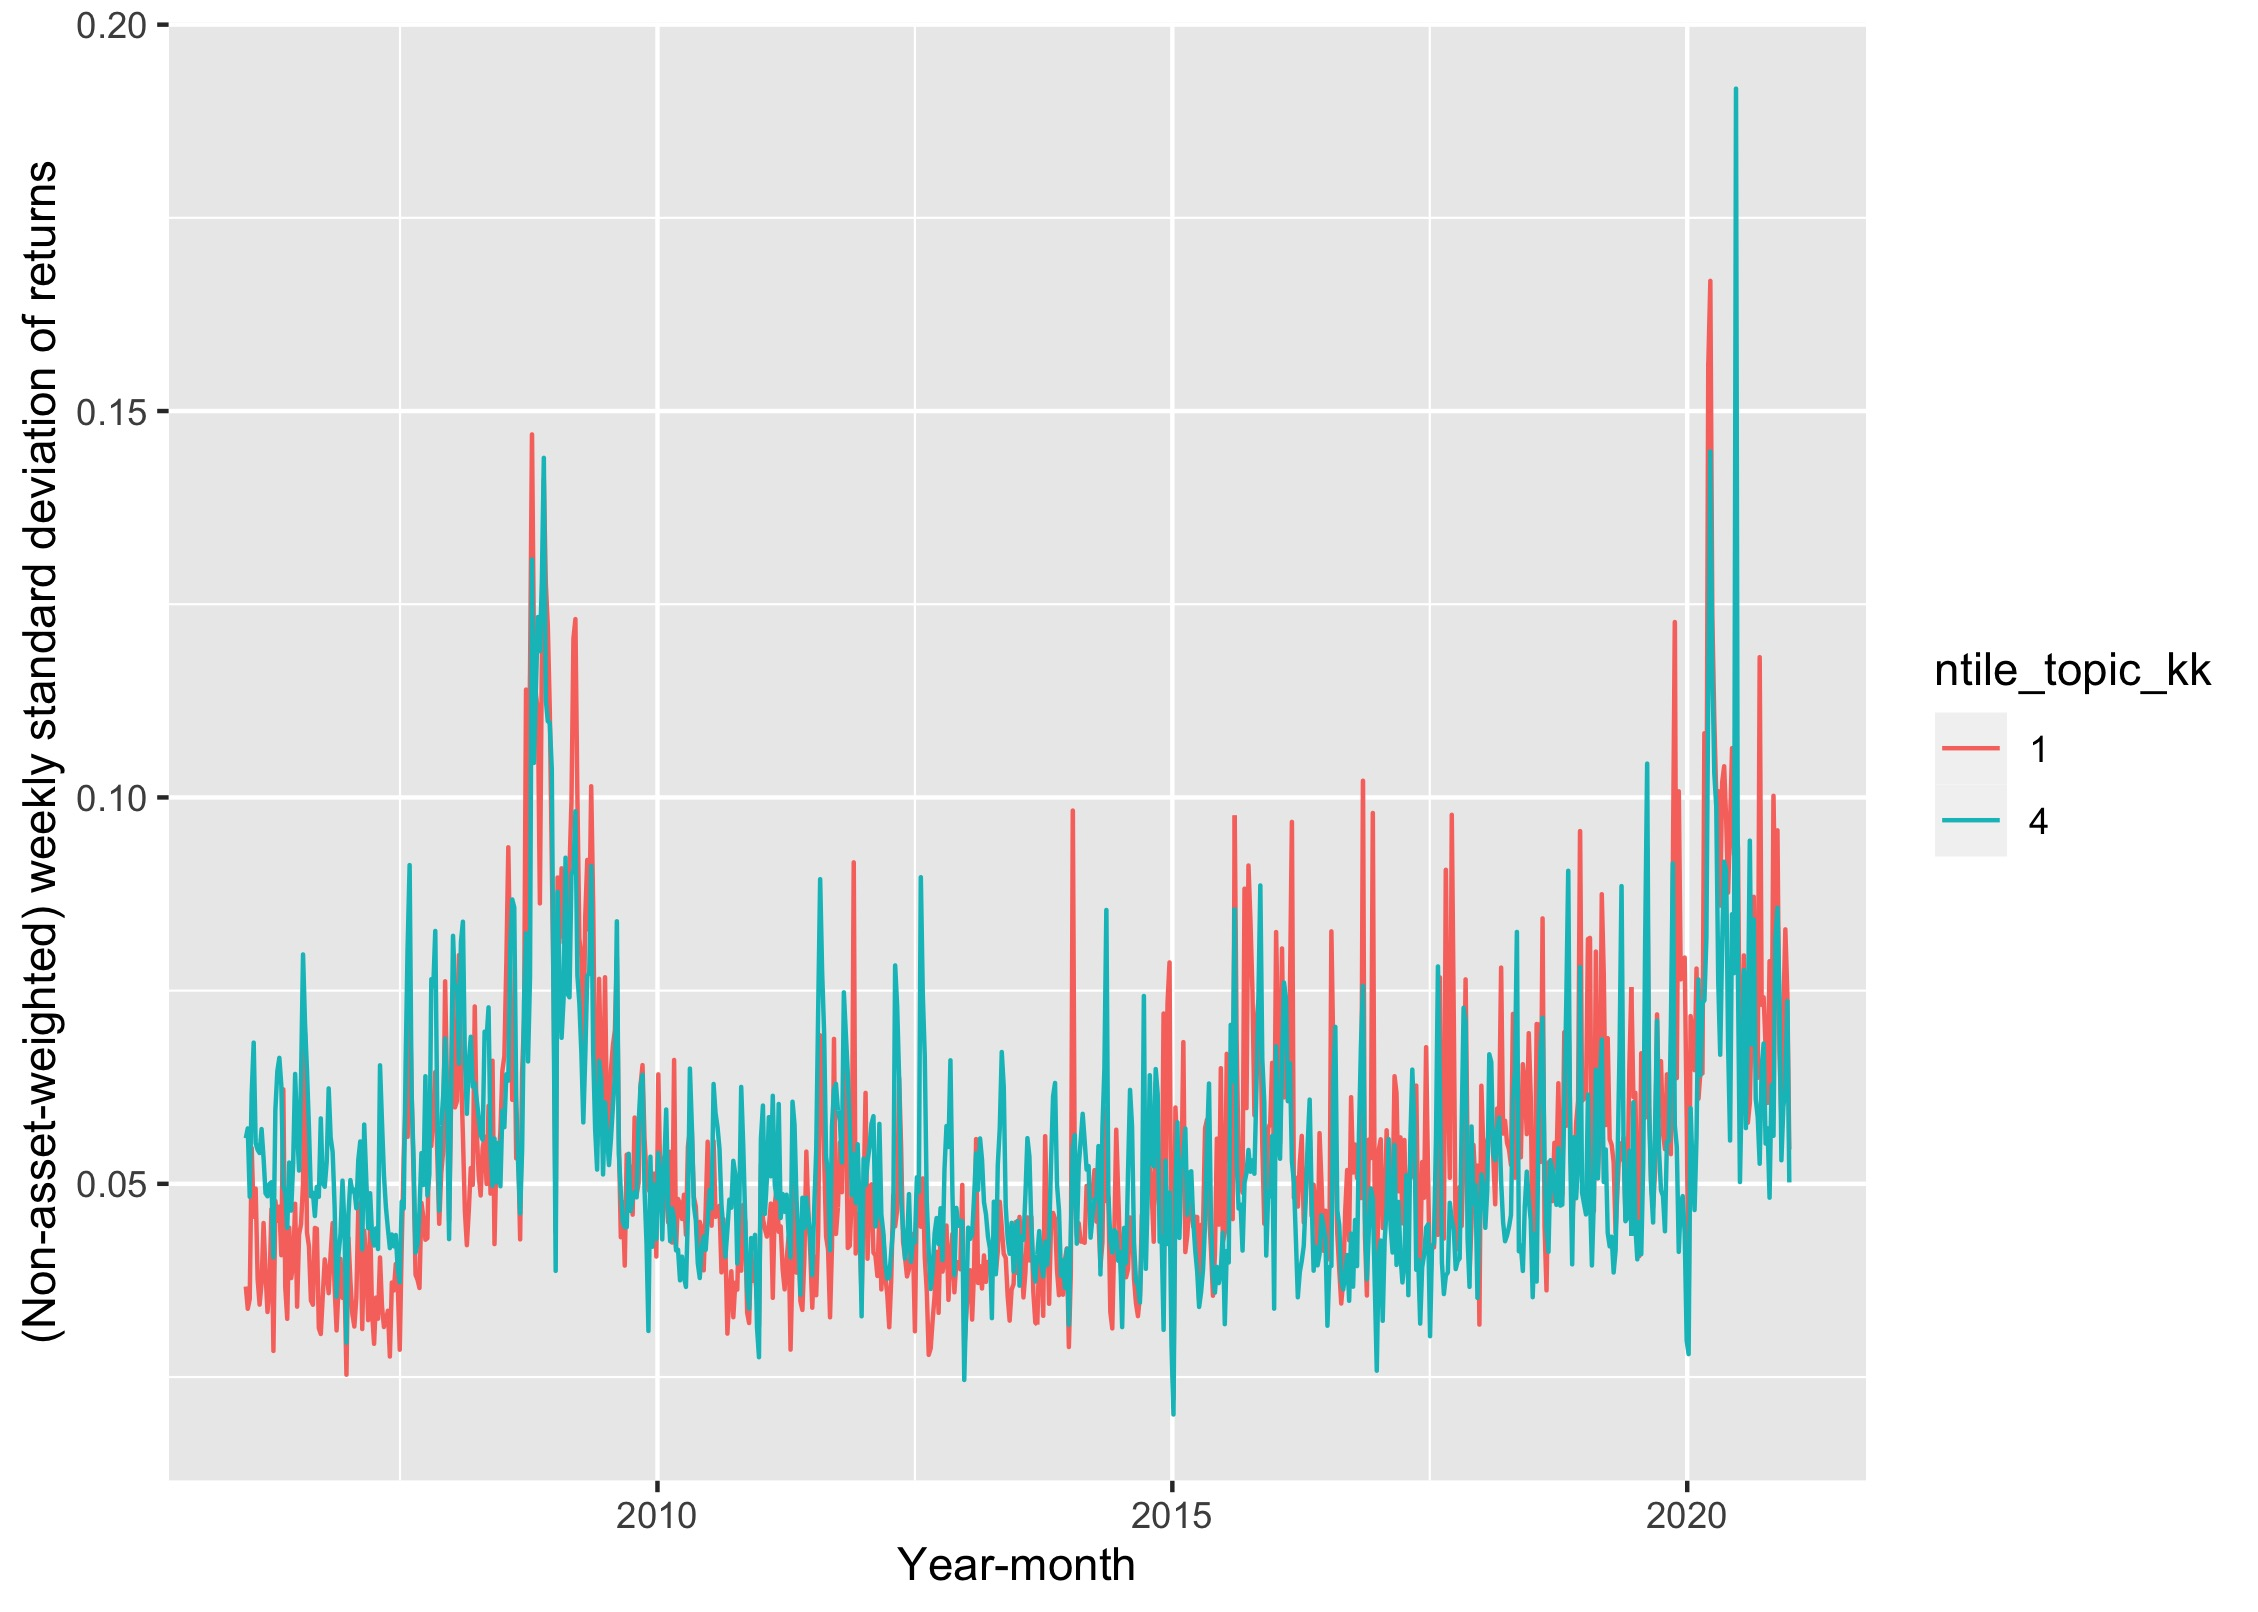
\includegraphics[width=0.8\textwidth]{\ffo/wsdr.jpg}
			\label{fig:wsdr}
			\caption{Weekly standard deviation of returns within groups, grouped by maximum topic. Higher KK risk is associated with higher return volatility}
\end{figure}


The study investigates the heterogeneity in kurtosis patterns across different topics, focusing on the impact of innovation activities on financial metrics. It identifies a correlation between innovation and increased cash flow volatility, which manifests as fatter tails in return distributions. The analysis involves calculating the kurtosis of daily returns for each firm on a yearly basis and averaging these kurtoses annually for each topic. A significant observation is that firms with a high level of knowledge intensity tend to exhibit consistently higher kurtosis compared to their peers, a trend that has been evident since 2006. This relationship is visually represented in the study through Figure \ref{fig:kurtosis_maxtopic}, which displays the weekly standard deviation of returns by maximum topic, providing a clear illustration of the varying kurtosis patterns.

\begin{figure}[h!]
\centering
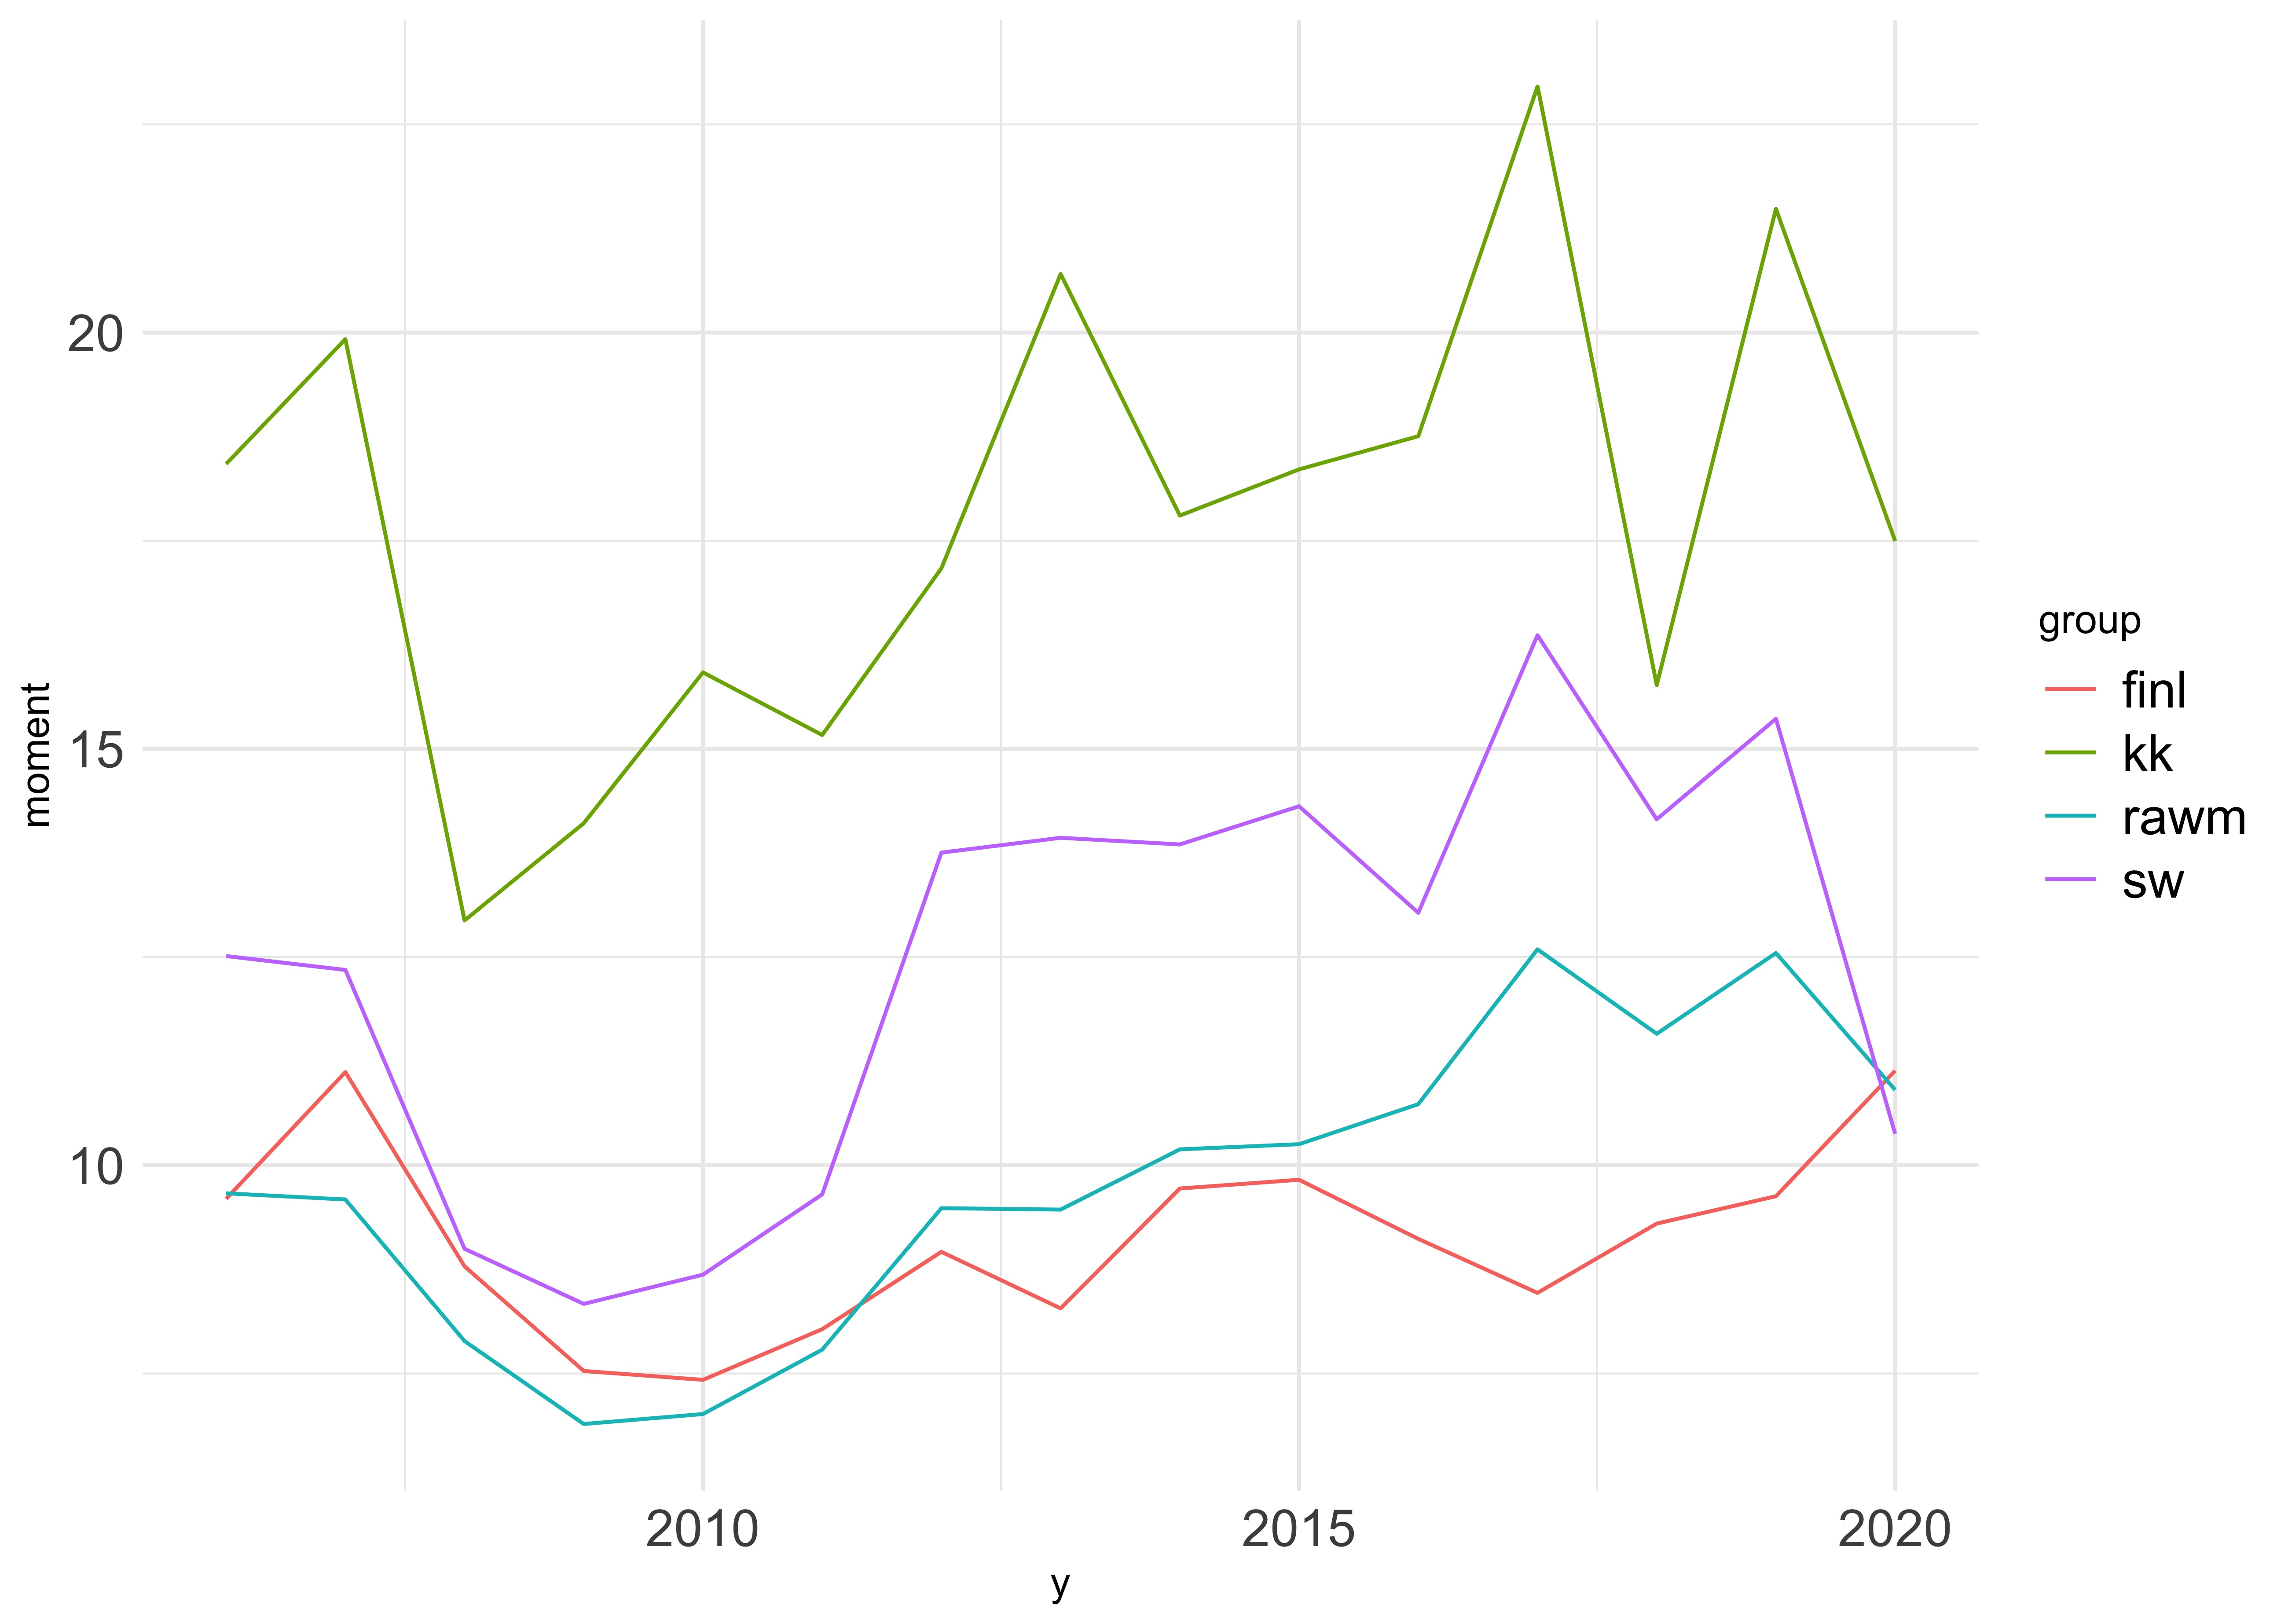
\includegraphics[width=0.9\textwidth]{\ffo/kurtosis_maxtopic.jpg}
\caption{Weekly Standard Deviation of Returns by Maximum Topic}
\label{fig:kurtosis_maxtopic}
\end{figure}

Furthering the analysis, the study examines the variation in kurtosis across quartiles of \tkk. This aspect focuses on how kurtosis fluctuates annually within categorized groups based on their quartile positioning in \tkk. A consistent and notable trend emerges from the data: as one moves to higher quartiles each year, kurtosis correspondingly increases. This pattern indicates a clear correlation between higher levels of self-reported knowledge capital risk and more pronounced tail risk in returns. This relationship is visually captured in Figure \ref{fig:kurtosis_ntile}.

\begin{figure}[h!]
\centering
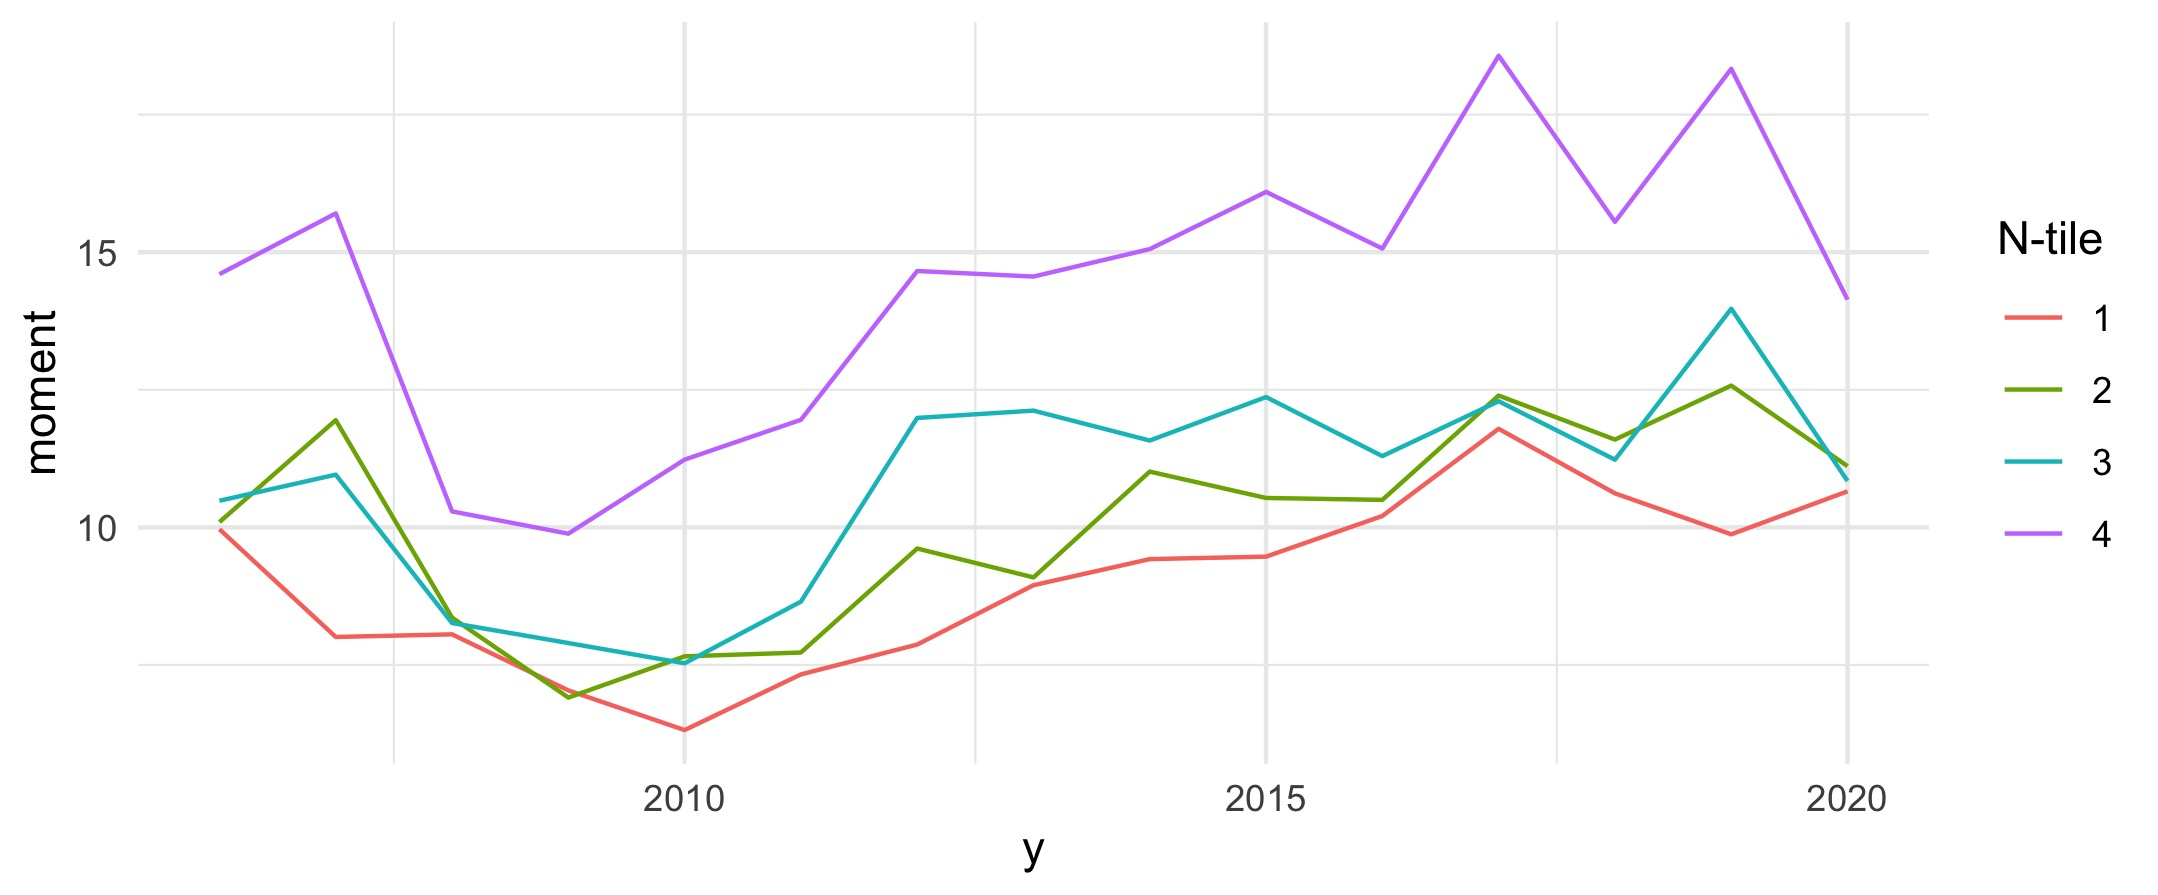
\includegraphics[width=0.9\textwidth]{\ffo/kurtosis_ntile.jpg}
\caption{Weekly Standard Deviation of Returns by $Topic\_{kk}$ Quartiles}
\label{fig:kurtosis_ntile}
\end{figure}

In the estimation of the knowledge risk premium \(\widehat{\lambda}_{kk}\), a two-stage approach is employed following the methodology outlined in \cite{Goyal2012-ct}. This involves the formation of 24 portfolios, expanding on the framework established by \cite{Fama1993-da}. The portfolios are categorized based on firm size (divided by NYSE's median), the MB ratio (divided by NYSE's 30th and 70th percentiles), and the quartiles of \(topic\_kk\). These portfolios are rebalanced every 26th calendar week.

For each portfolio \(i\) and week \(t\), beta estimates are obtained through time-series regressions:

\begin{align*}
    R_{it} - R_{F,t} &= a_i + \beta_{M, i}(R_{M,t} - R_{F,t}) + \beta_{SMB, i} SMB_t \\
    &+ \beta_{HML, i} HML_t + \beta_{KKHML, i} KKHML_t + \varepsilon_{i,t}
\end{align*}

Data for \(R_{F,t}\), \(SMB_t\), \(HML_t\), and \(R_{M,t} - R_{F,t}\) are sourced weekly from Kenneth French's database. The \(KKHML_t\) factor, representing differential excess return, is calculated as the difference between the returns of value-weighted portfolios in the lowest and highest quartiles of KK. Furthermore, a cross-sectional regression of average returns on betas is conducted:

\begin{align}
    \bar{R}_T = \widehat{B} \lambda + \alpha
\end{align}

The summarized findings and detailed analysis are presented in the summary table, integrated from an external file:


% Table created by stargazer v.5.2.2 by Marek Hlavac, Harvard University. E-mail: hlavac at fas.harvard.edu
% Date and time: Thu, Jan 25, 2024 - 16:57:10
% Requires LaTeX packages: dcolumn 
\begin{table}[!htbp] \centering 
  \caption{Regression Summary} 
  \label{} 
\begin{tabular}{@{\extracolsep{5pt}}lD{.}{.}{-3} D{.}{.}{-3} } 
\\[-1.8ex]\hline 
\hline \\[-1.8ex] 
 & \multicolumn{2}{c}{\textit{Dependent variable:}} \\ 
\cline{2-3} 
\\[-1.8ex] & \multicolumn{2}{c}{Average returns} \\ 
\\[-1.8ex] & \multicolumn{1}{c}{(1)} & \multicolumn{1}{c}{(2)}\\ 
\hline \\[-1.8ex] 
 kkrhml & -0.001^{***} &  \\ 
  & (0.0004) &  \\ 
  & & \\ 
 HML & -0.003^{***} & -0.003^{***} \\ 
  & (0.0005) & (0.001) \\ 
  & & \\ 
 SMB & -0.0001 & 0.0001 \\ 
  & (0.0004) & (0.0004) \\ 
  & & \\ 
 Mkt.RF & 0.002 & 0.003^{*} \\ 
  & (0.002) & (0.002) \\ 
  & & \\ 
 Constant & 0.001 & -0.001 \\ 
  & (0.002) & (0.002) \\ 
  & & \\ 
\hline \\[-1.8ex] 
Observations & \multicolumn{1}{c}{36} & \multicolumn{1}{c}{36} \\ 
R$^{2}$ & \multicolumn{1}{c}{0.614} & \multicolumn{1}{c}{0.469} \\ 
Adjusted R$^{2}$ & \multicolumn{1}{c}{0.564} & \multicolumn{1}{c}{0.419} \\ 
Residual Std. Error & \multicolumn{1}{c}{0.00001 (df = 31)} & \multicolumn{1}{c}{0.00001 (df = 32)} \\ 
F Statistic & \multicolumn{1}{c}{12.322$^{***}$ (df = 4; 31)} & \multicolumn{1}{c}{9.405$^{***}$ (df = 3; 32)} \\ 
\hline 
\hline \\[-1.8ex] 
\textit{Note:}  & \multicolumn{2}{r}{$^{*}$p$<$0.1; $^{**}$p$<$0.05; $^{***}$p$<$0.01} \\ 
\end{tabular} 
\end{table} 


%\insertfigure{wsdr_byg}{Weekly Standard Deviation of Returns Within Groups, Indicating Variations Across Different Topics}{0.7}

\section{Conclusion}

This study is ongoing, with numerous opportunities for enhancement and further exploration. For instance, the hyperparameter selection process could be optimized, potentially through cross-validation techniques. Existing benchmarks for the choice of $k$, such as perplexity, are also being considered for testing.

In addition, the current methodology might evolve towards supervised models. For example, a prior for $Topic_{kk}$ could be imposed, comprising specific words such as ``patents" or ``intellectual property." So far, the learning process has been completely unsupervised.

Another area of interest is testing whether the derived topics can serve as factors in asset pricing models or if they can clarify any anomalies. Moreover, it would be valuable to examine whether the language associated with $Topic_{kk}$ has transformed over time. These areas of focus highlight the promising possibilities for further research and development in this study.

%\insertfigure{heatmap_patents}{Correlation matrix between topics and patent intensity}{0.7}
%
%\FloatBarrier
%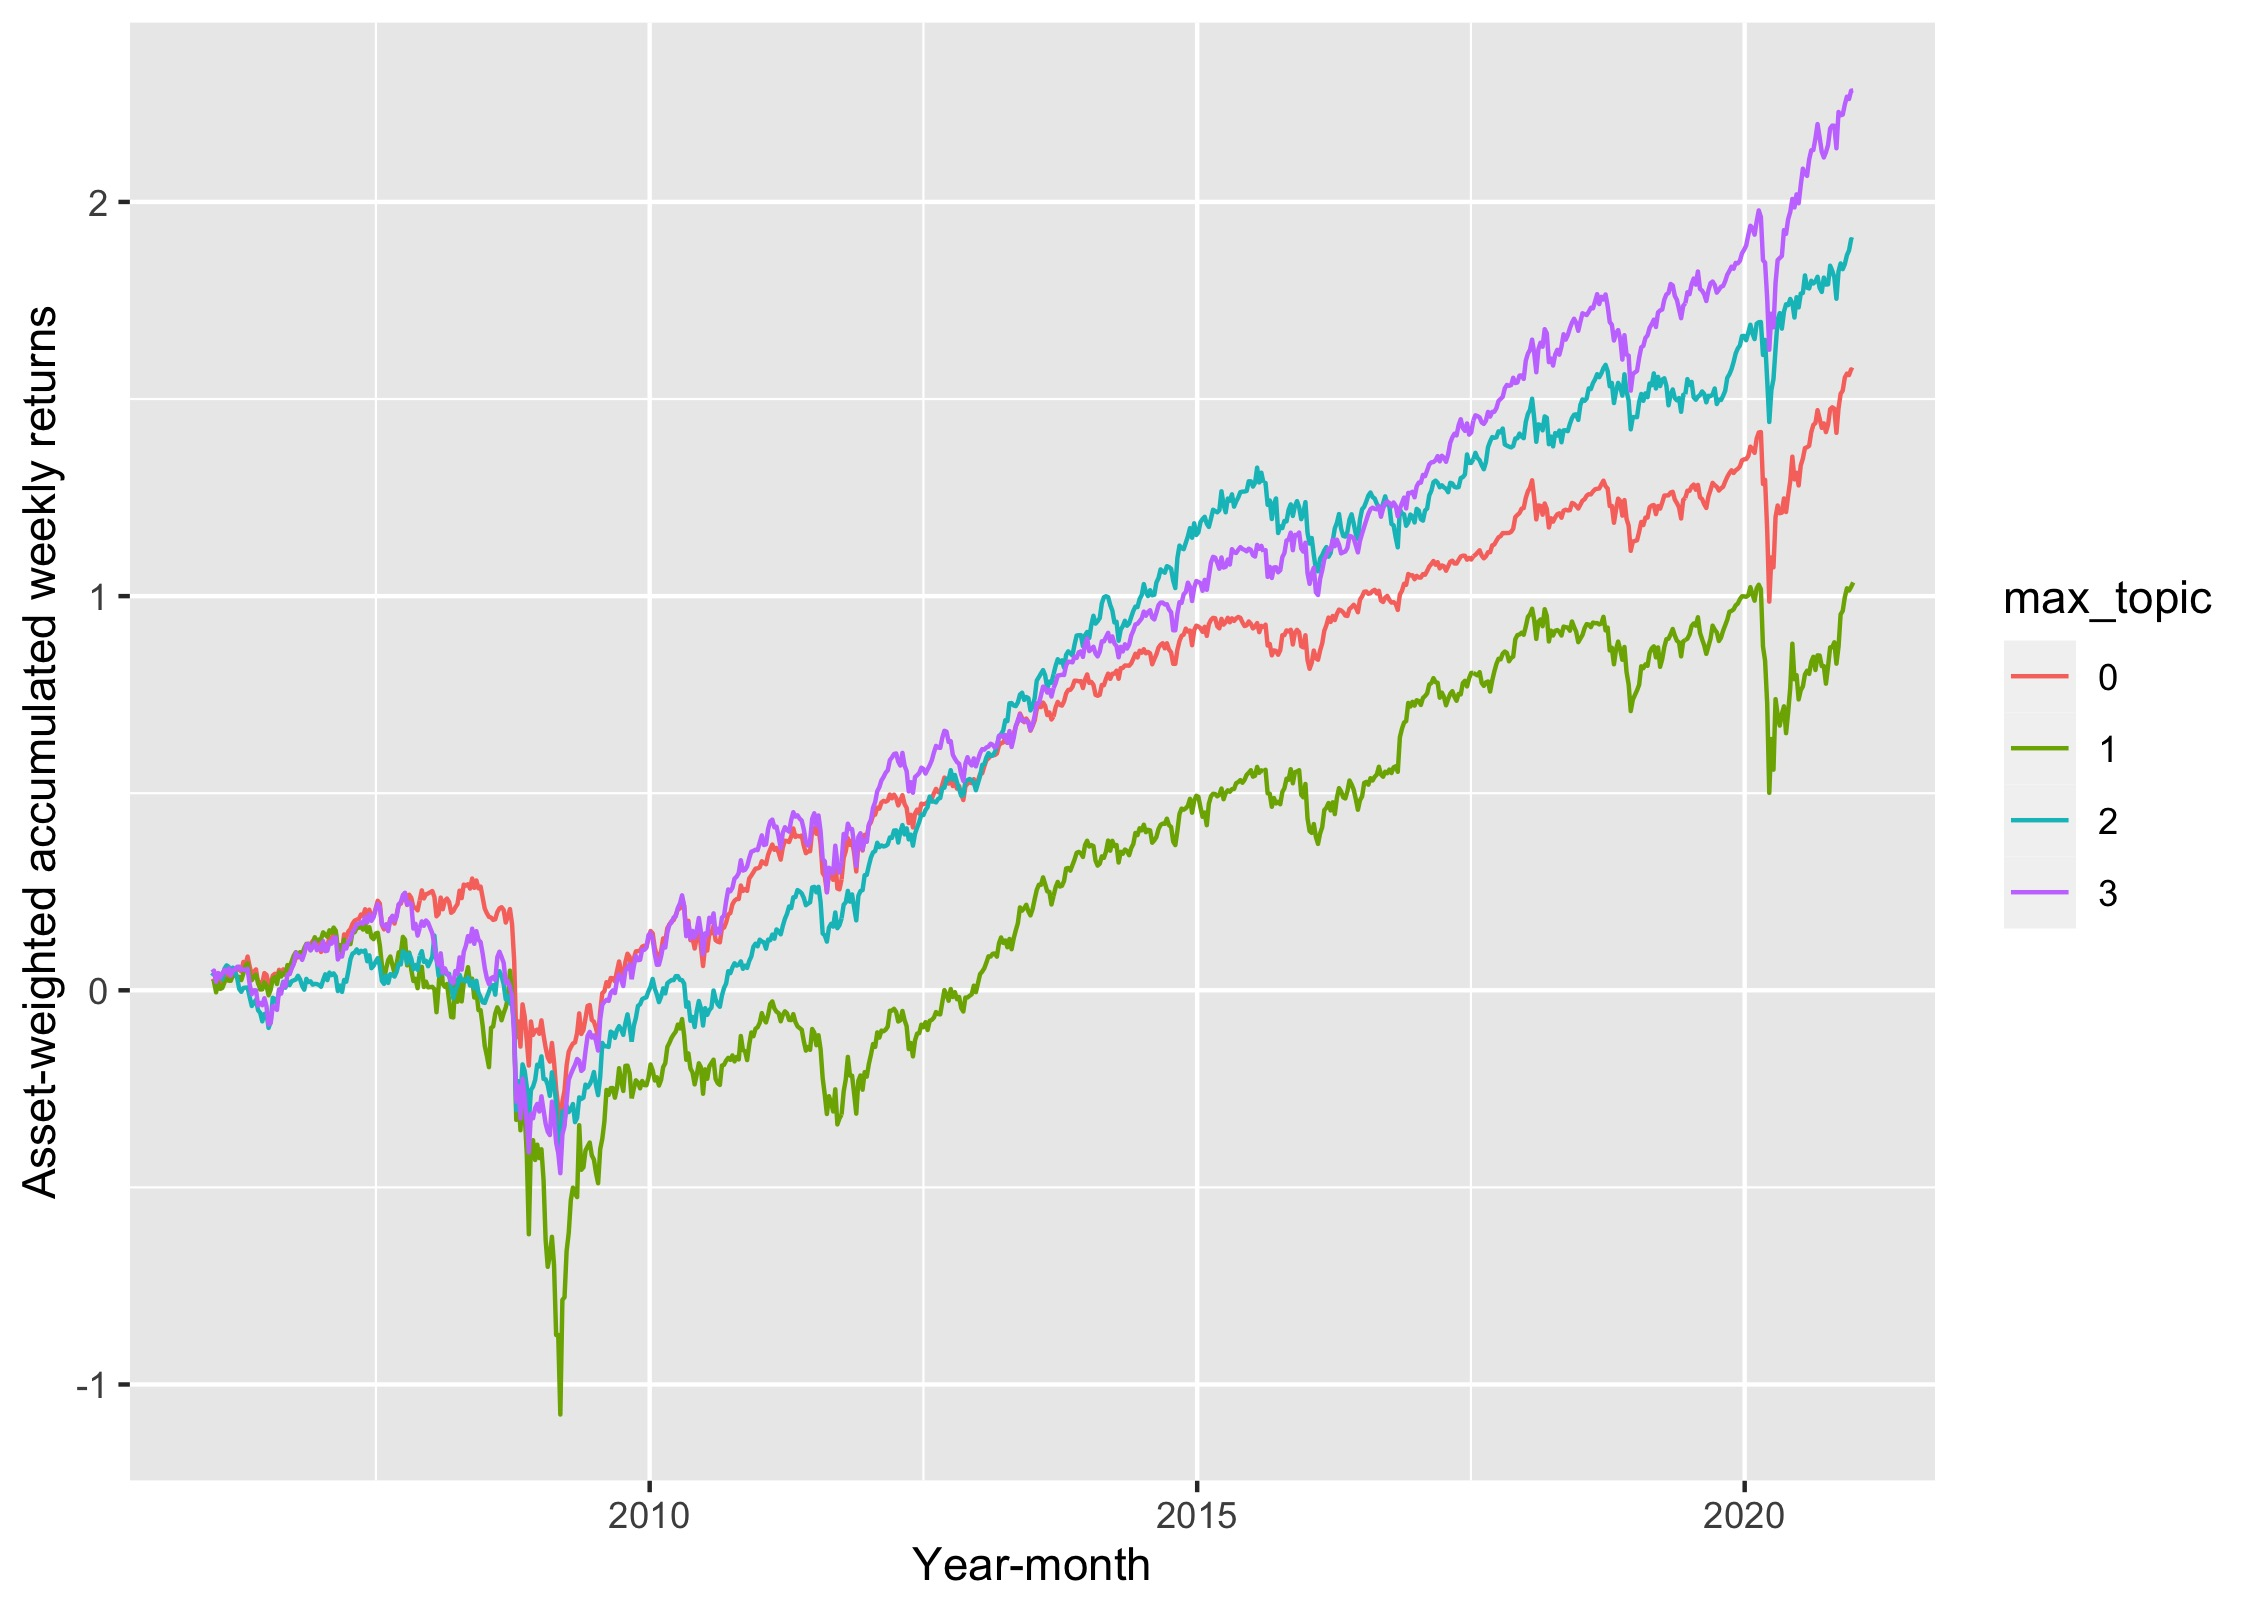
\includegraphics[width=0.6\textwidth]{\ffo/awawr_byg.jpg}
%\FloatBarrier
%
%\insertfigure{stackedplot_at}{Stacked plot of firms' total assets in the upper quartile of KK topic intensity}{0.7}
%
%\insertfigure{stackedplot_n}{-}{0.7}
%
%\insertfigure{topicvsikpt_hm}{-}{0.7}
%
%\insertfigure{topicvskkpt_hm}{-}{0.7}

\bibliography{mylibrary2}

\section*{Appendix A: Extracting risk factors' data}
10-K documents are retrieved from EDGAR as HTML files.
I extract the item 1A information from each 10-K using HTML parsing and \texttt{BeautifulSoup}, and remove punctuation and numbers.

\section*{Appendix B: Text conversion to bag-of-words}
\label{bow}

After filtering the firms, I employ the \texttt{spacy} Python library to conduct lemmatization on all the refined texts. Lemmatization transforms words into their base form, ensuring consistent semantics. As an illustration, words such as ``take'', ``took'', and ``taken'' are standardized to ``take''. To do so, \texttt{spacy} leverages WordNet---a comprehensive English lexical database curated by Princeton University.

To extract significant collocations---like ``patent application''---which provide richer semantic insights than individual words, this research adopts the collocation detection method outlined in \cite{Mikolov2013-be}. This methodology yields pertinent bigrams and trigrams. A minimum occurrence threshold of 5 ensures that only the most statistically relevant combinations are incorporated into the dictionary.

This research compiles the entirety of discovered words, bigrams, and trigrams to formulate a dictionary. 

Lastly, the texts are transformed into a bag-of-words model using both the dictionary and the n-gram processed texts. In this representation, each word's frequency in a document, denoted as \(c_{ij}\), is preserved, but the sequence of words is omitted, leading to the final depiction of the corpus.

\begin{figure}[H] % Use [H] to force the figure to be here
  \centering
  \begin{subfigure}{0.45\textwidth}
    \centering
    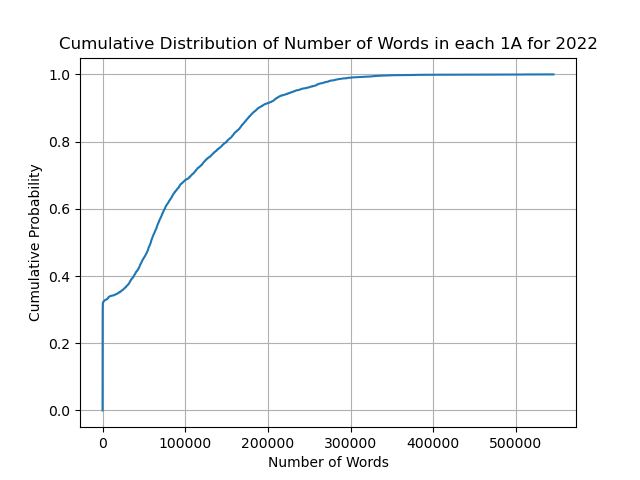
\includegraphics[width=\textwidth]{cdf_words}
	\caption{Cumulative Distribution of Number of Words}	
    \label{fig:figure1}
  \end{subfigure}
  \hfill
  \begin{subfigure}{0.45\textwidth}
    \centering
    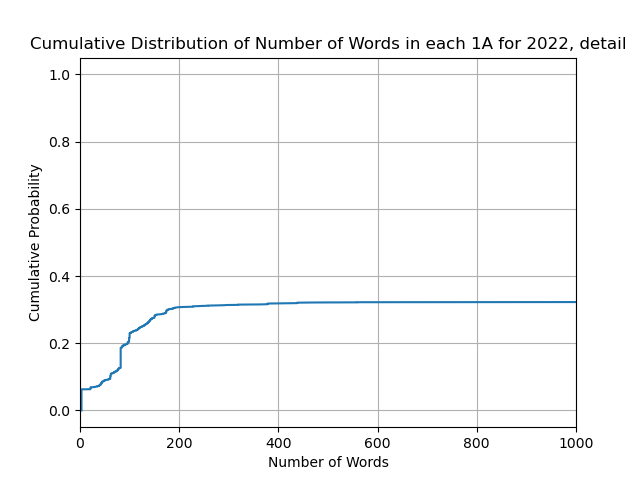
\includegraphics[width=\textwidth]{cdf_words_zoom}
	\caption{Cumulative Distribution of Number of Words, Zoom}
    \label{fig:figure2}
  \end{subfigure}
  \caption{Cumulative Distribution of Number of Words in 2022}
  \label{fig:cdf}
\end{figure}


\section*{Appendix C: Correlation of topic loadings with previous measures of knowledge capital intensity from the literature}

Figure \ref{fig:heatmap} presents a correlation matrix that delineates the relationship between the intensity of each topic and the average skill level of employees within a narrowly-defined industry, in accordance with the definition given by Belo et al. (2017). These authors define 'Skill' as the proportion of industry workers engaged in occupations that demand a high degree of training and preparation.

The determination of whether an occupation is high-skill is informed by the Specific Vocational Preparation (SVP) level for each occupation. This data is sourced from the 1991 edition of the Dictionary of Occupational Titles (DOT), published by the U.S. Department of Labor. 

In Belo et al.'s (2017) classification, an occupation is considered high-skill if it possesses an SVP level of 7 or greater. This level implies a requirement of two or more years of preparation. Occupations failing to meet this threshold are classified as low-skill.

\insertfigure{heatmap}{Correlation Matrix Showcasing the Relationship between Topic Intensity and Industry Employee Skill Level}{0.7}

The second component of the analysis, shown in Figure \ref{fig:firmsbypat_hm}, computes the co-occurrences of quartiles for $Topic_{kk}$ and the accumulated patent-related market value within firms, in alignment with the methodology proposed by \cite{Kogan2017-fx}. \cite{Kogan2017-fx} leveraged stock market data to estimate the value of individual patents filed by public corporations since 1926. 

 In Figure \ref{fig:firmsbypat_hm}, the vertical axis signifies annually assigned quartiles of the ratio between Accumulated Patent Value and Total Assets. The results imply a clear correlation between elevated accumulated patent value and increased loadings of $Topic_{kk}$. A basic correlation analysis between average patent intensity and different topics is shown in Figure \ref{fig:heatmap_patents}.

\insertfigure{heatmap_patents}{Quartiles of \tkk vs. quartiles of accumulated total patent market value}{0.7}

\end{document} 